\subsection{有限生成模的结构}

定理2.——设A为主理想整环，则每个有限生成的A-模E都同构于有限多个（m 个）循环模 \(A/a_{k}\) 的直和，其中 \(a_{k}\) 是 A 的理想（其中某些可以为零），满足 \(a_{1} \subset a_{2} \subset \ldots \subset a_{m} \neq A\)，并且这些理想由上述条件唯一确定。

如果 E 可由 q 个元素生成，则它同构于一个商模 L/M，其中 \(L = A^{q}\)（II，第 218 页）。由于 M 具有有限秩 \(n \leqslant q\)（VII，第 15 页，命题 1），定理 1（VII，第 18 页）的条件得到满足。于是在定理 1 的记号下，L/M 同构于 \(L'\)（\(M'\) 在 L 中的一个补）与挠模 \(M'/M\) 的直和。模 \(L'\) 是秩为 p = q − n 的自由模，故同构于 \(A^{p}\)。若 r 是使 \(A\alpha_{r} \neq A\) 的最小指标，则 \(M'/M\) 同构于诸模 \(A/A\alpha_{i}\)（\(r \leqslant i \leqslant n\)）的直和。于是，若取 \(m = p + (n - r + 1)\)、\(\mathfrak{a}_{k} = (0)\)（\(1 \leqslant k \leqslant p\)）以及 \(\mathfrak{a}_{p+j} = A\alpha_{n-j+1}\)（\(1 \leqslant j \leqslant n - r + 1\)），则所述条件即得到满足。唯一性由 VII 第 16 页的推论得出。

\pandocbounded{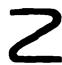
\includegraphics[keepaspectratio]{images/part003_91527dd3.jpg}}

推论 1. --- 主理想整环上的每个有限生成模 E 都是 E 的挠子模与一个自由模的直和。

E 的挠子模一般有若干个不同的补。例如，若 \(E = \mathbf{Z} \times (\mathbf{Z}/(2))\)，则 E 的挠子模为 \(\{0\} \times (\mathbf{Z}/(2))\)；它有一个补 \(Z \times \{0\}\)，也有由所有形如 \((n, \bar{n})\) 的元素组成的子模，其中 n 遍历 Z，\(\bar{n}\) 是 n 模 2 的剩余类。

推论 2. --- 主理想整环上的每个无挠有限生成模都是有限秩的自由模。

这直接由推论1得出。

\pandocbounded{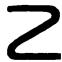
\includegraphics[keepaspectratio]{images/part003_b18cf4bc.jpg}}

模为有限生成的这一条件是本质的。例如，A 的分式域 K 的加法群作为 A-模是无挠的；然而当 \(A \neq K\) 时它不是自由模，因为一方面 K 的任意两个元素都有一个公因子，另一方面 K 不是循环 A-模，否则 \(K = ab^{-1}A\)（\(a, b \in A\)），从而 \(b^{-2} = acb^{-1}\)（\(c \in A\)），于是 \(b^{-1} = ac \in A\)，即 K = A。

定义2. --- 在定理2的记号与假设下，理想 \(\mathfrak{a}_k\) 称为模E的不变因子。

正如定义 1（VII，第 19 页）那样，当 A = Z 或 A = K{[}X{]} 时，理想 \(a_{k}\) 的典范生成元（正整数或首一多项式）（滥用术语）也称为有限生成模 E 的一个不变因子。

\pandocbounded{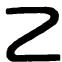
\includegraphics[keepaspectratio]{images/part003_8ba9a087.jpg}}

我们必须小心，不要将模 E 的不变因子与自由模 L 的子模 M 关于模 L 的不变因子（定义 1）混淆。

